\newpage
\newsection{Event Sourcing}
\begin{center}
	\emph{"Event Sourcing ensures that all changes to application are stored as a sequence of events."} \\
\end{center}

You can query the events, use the event log to reconstruct past states and adjust the state to cope with retroactive changes.\\
The core idea of event sourcing is that whenever we make a change to the state of a system, we record that state change as an event and we can confidently rebuild the system state by reprocessing the events at any time in the future.\\
Before storing the event you must validate it because you don't have to store events that generate errors or exceptions.\\ 
When working with an event log can be useful to build snapshots of the working copy so that you don't have to process all the events when you rebuild the system or every time you need to query the database. For this reason when a new event is stored triggers another function to update the views.\\
Event sourcing can be used to:
\begin{itemize}
	\item \textbf{Complete Rebuild}: you can completely discard the application state  and rebuild it by re-running the events from the event store on an empty application.
	\item \textbf{Temporal Query}: you can determine the application state at any point in time. This can be used considering multiple time-lines (like branching in a VCS).
	\item \textbf{Event Replay}: if you find that a past event was incorrect, you can replaying from then with the correct event. The same technique can handle events received in the wrong sequence with systems that communicate with asynchronous messaging.
	
\end{itemize}

\subsection{Event store}
Event store is a database's table that contains all the events occurred from the begin.
With event sourcing the event store becomes the principal source of truth and the system state is completely derived from it. \\
Is essential that the table can't be modified and the events that are replayed don't have to be stored again. 
This because the event store can reach huge dimensions and we must avoid to overload it.\\
In a complex system with billions of users the best choice is to implement an event store table for each aggregate object in order to keep track of the events that occurred to a single entity. In this way there are more event stores but this tables have less entries and this increase the speed of a query operation.

\subsubsection{Event object}
Each event stored in the table is a JSON object and respect this format:
\begin{itemize}
	\item \textbf{EventId}: is a UUID;
	\item \textbf{Payload}:	JSON object which contains all the information about the event;
	\item \textbf{Aggregate}: type of the aggregate that the event refers to;
	\item \textbf{ExecutionQueue}: name of the execution queue used to execute the event;
	\item \textbf{Timestamp}: number to know the execution order of the events.
\end{itemize}

\begin{figure} [H]
	\centering
	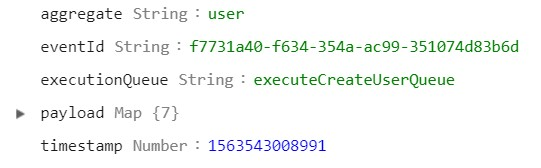
\includegraphics[scale=1.2]{../Img/event_object}
	\caption{Event object item}\label{}
\end{figure}


